%% This file was auto-generated by IPython.
%% Conversion from the original notebook file:
%% /home/will/IpythonNotebook/VariationPlots.ipynb
%%
\documentclass[11pt,english]{article}

%% This is the automatic preamble used by IPython.  Note that it does *not*
%% include a documentclass declaration. The documentclass is added at runtime
%% to the overall document.

\usepackage{amsmath}
\usepackage{amssymb}
\usepackage{graphicx}
\usepackage{ucs}
\usepackage[utf8x]{inputenc}

% needed for markdown enumerations to work
\usepackage{enumerate}

% Slightly bigger margins than the latex defaults
\usepackage{geometry}
\geometry{verbose,tmargin=3cm,bmargin=3cm,lmargin=2.5cm,rmargin=2.5cm}

% Define a few colors for use in code, links and cell shading
\usepackage{color}
\definecolor{orange}{cmyk}{0,0.4,0.8,0.2}
\definecolor{darkorange}{rgb}{.71,0.21,0.01}
\definecolor{darkgreen}{rgb}{.12,.54,.11}
\definecolor{myteal}{rgb}{.26, .44, .56}
\definecolor{gray}{gray}{0.45}
\definecolor{lightgray}{gray}{.95}
\definecolor{mediumgray}{gray}{.8}
\definecolor{inputbackground}{rgb}{.95, .95, .85}
\definecolor{outputbackground}{rgb}{.95, .95, .95}
\definecolor{traceback}{rgb}{1, .95, .95}

% Framed environments for code cells (inputs, outputs, errors, ...).  The
% various uses of \unskip (or not) at the end were fine-tuned by hand, so don't
% randomly change them unless you're sure of the effect it will have.
\usepackage{framed}

% remove extraneous vertical space in boxes
\setlength\fboxsep{0pt}

% codecell is the whole input+output set of blocks that a Code cell can
% generate.

% TODO: unfortunately, it seems that using a framed codecell environment breaks
% the ability of the frames inside of it to be broken across pages.  This
% causes at least the problem of having lots of empty space at the bottom of
% pages as new frames are moved to the next page, and if a single frame is too
% long to fit on a page, it will completely stop latex from compiling the
% document.  So unless we figure out a solution to this, we'll have to instead
% leave the codecell env. as empty.  I'm keeping the original codecell
% definition here (a thin vertical bar) for reference, in case we find a
% solution to the page break issue.

%% \newenvironment{codecell}{%
%%     \def\FrameCommand{\color{mediumgray} \vrule width 1pt \hspace{5pt}}%
%%    \MakeFramed{\vspace{-0.5em}}}
%%  {\unskip\endMakeFramed}

% For now, make this a no-op...
\newenvironment{codecell}{}

 \newenvironment{codeinput}{%
   \def\FrameCommand{\colorbox{inputbackground}}%
   \MakeFramed{\advance\hsize-\width \FrameRestore}}
 {\unskip\endMakeFramed}

\newenvironment{codeoutput}{%
   \def\FrameCommand{\colorbox{outputbackground}}%
   \vspace{-1.4em}
   \MakeFramed{\advance\hsize-\width \FrameRestore}}
 {\unskip\medskip\endMakeFramed}

\newenvironment{traceback}{%
   \def\FrameCommand{\colorbox{traceback}}%
   \MakeFramed{\advance\hsize-\width \FrameRestore}}
 {\endMakeFramed}

% Use and configure listings package for nicely formatted code
\usepackage{listingsutf8}
\lstset{
  language=python,
  inputencoding=utf8x,
  extendedchars=\true,
  aboveskip=\smallskipamount,
  belowskip=\smallskipamount,
  xleftmargin=2mm,
  breaklines=true,
  basicstyle=\small \ttfamily,
  showstringspaces=false,
  keywordstyle=\color{blue}\bfseries,
  commentstyle=\color{myteal},
  stringstyle=\color{darkgreen},
  identifierstyle=\color{darkorange},
  columns=fullflexible,  % tighter character kerning, like verb
}

% The hyperref package gives us a pdf with properly built
% internal navigation ('pdf bookmarks' for the table of contents,
% internal cross-reference links, web links for URLs, etc.)
\usepackage{hyperref}
\hypersetup{
  breaklinks=true,  % so long urls are correctly broken across lines
  colorlinks=true,
  urlcolor=blue,
  linkcolor=darkorange,
  citecolor=darkgreen,
  }

% hardcode size of all verbatim environments to be a bit smaller
\makeatletter
\g@addto@macro\@verbatim\small\topsep=0.5em\partopsep=0pt
\makeatother

% Prevent overflowing lines due to urls and other hard-to-break entities.
\sloppy

\begin{document}

\section{Examination of HIV Variation}
In an effort to examine the amount of genetic variation from
longitudinal visits of well-controlled patients. We are determining the
number of mutations that occur in the LTR over a set of consecutive
visits in which the patient has maintained a Viral-Load \textless{}100
copies/mL and a CD4 count \textgreater{} 250 cells/mL.

\begin{codecell}
\begin{codeinput}
\begin{lstlisting}
from __future__ import division
from pandas import *
import os, os.path
import sys
import numpy as np

sys.path.append('/home/will/HIVReportGen/AnalysisCode/')
sys.path.append('/home/will/PySeqUtils/')
os.chdir('/home/will/HIVVariation/')
\end{lstlisting}
\end{codeinput}
\end{codecell}
\begin{codecell}
\begin{codeinput}
\begin{lstlisting}
from GeneralSeqTools import call_muscle
\end{lstlisting}
\end{codeinput}
\end{codecell}
\subsection{Data Extraction}
Using the Redcap and sequence data up until 1/16/2013.

\begin{codecell}
\begin{codeinput}
\begin{lstlisting}
store = HDFStore('/home/will/HIVReportGen/Data/SplitRedcap/2013-01-16/EntireCohort.hdf')
redcap_data = store['redcap']
seq_data = store['seq_data']

t = redcap_data['Event Name'].dropna().apply(lambda x: x.split(' - ')[0])
t.unique()
redcap_data['Patient visit number'] = redcap_data['Patient visit number'].combine_first(t)


\end{lstlisting}
\end{codeinput}
\end{codecell}
\begin{codecell}
\begin{codeinput}
\begin{lstlisting}
def VisitType(row):
    
    if row['ART'] == 'naive':
        return 'naive'
    elif (row['CD4'] >= 250) & (row['VL']<=100):
        return 'controlled'
    else:
        return 'wild'
    
\end{lstlisting}
\end{codeinput}
\end{codecell}
\begin{codecell}
\begin{codeinput}
\begin{lstlisting}
wanted_cols = ['Patient ID', 'Patient visit number', 
                'Date of visit', 'Latest CD4 count (cells/uL)', 
                'Latest viral load', 'Current ART status']
wanted_redcap = redcap_data[wanted_cols]
data = merge(wanted_redcap, seq_data[['LTR']],
            left_on = ['Patient ID', 'Patient visit number'],
            right_index = True, how = 'inner').dropna()
data = data.rename(columns= {
                                'Patient visit number':'VisitNum',
                                'Date of visit':'Date',
                                'Latest CD4 count (cells/uL)':'CD4',
                                'Latest viral load':'VL',
                                'Current ART status':'ART'
                            })

data['VisitType'] = data.apply(VisitType, axis = 1)
print 'Valid samples from Redcap/Sequencing'
print data
\end{lstlisting}
\end{codeinput}
\begin{codeoutput}
\begin{verbatim}
Valid samples from Redcap/Sequencing
<class 'pandas.core.frame.DataFrame'>
Int64Index: 954 entries, 1 to 1397
Data columns:
Patient ID    954  non-null values
VisitNum      954  non-null values
Date          954  non-null values
CD4           954  non-null values
VL            954  non-null values
ART           954  non-null values
LTR           954  non-null values
VisitType     954  non-null values
dtypes: float64(2), object(6)
\end{verbatim}
\end{codeoutput}
\end{codecell}
\begin{codecell}
\begin{codeinput}
\begin{lstlisting}
from copy import deepcopy

def filter_to_runs(df, visit_type = True):
    
    min_run = 3
    
    ndf = df.copy()
    ndf.sort('Date')
    ndf['RunLen'] = np.nan
    ndf['DaysFromControlled'] = np.nan
    
    crun = []
    mrun = []
    for ind, row in ndf.iterrows():
        if row['VisitType'] == visit_type:
            crun.append(ind)
        else:
            if len(crun) > len(mrun):
                mrun = deepcopy(crun)
                crun = []
    
    if len(mrun) >= min_run:
        ndf['RunLen'][mrun] = len(mrun)
        deltas = (ndf['Date'][mrun] - ndf['Date'][mrun[0]])
        ndf['DaysFromControlled'][mrun] = deltas.map(lambda x:x.days)
        
    return ndf

controlled_data = data.groupby('Patient ID', 
                                as_index = False).apply(filter_to_runs, 
                                visit_type = 'controlled').dropna()
wild_data = data.groupby('Patient ID', 
                        as_index = False).apply(filter_to_runs, 
                        visit_type = 'wild').dropna()
naive_data = data.groupby('Patient ID', 
                          as_index = False).apply(filter_to_runs, 
                          visit_type = 'naive').dropna()
\end{lstlisting}
\end{codeinput}
\end{codecell}
\begin{codecell}
\begin{codeinput}
\begin{lstlisting}
hxb2_ltr = """TGGAAGGGCTAATTTACTCCCAAAAAAGACAAGATATCCTTGATCTGTGGGTC
TACCACACACAAGGCTACTTCCCTGATTGGCAGAACTACACACCAGGGCCAGG
GATCAGATATCCACTGACCTTTGGATGGTGCTTCAAGCTAGTACCAGTTGAGC
CAGAGAAGGTAGAAGAGGCCAATGAAGGAGAGAACAACAGCTTGTTACACCCT
ATGAGCCTGCATGGGATGGAGGACCCGGAGAAAGAAGTGTTAGTGTGGAAGTT
TGACAGCCGCCTAGCATTTCATCACATGGCCCGAGAGCTGCATCCGGAGTACT
ACAAGGACTGCTGACATCGAGCTTTCTACAAGGGACTTTCCGCTGGGGACTTT
CCAGGGAGGCGTGGCCTGGGCGGGACTGGGGAGTGGCGAGCCCTCAGATGCTG
CATATAAGCAGCTGCTTTTTGCCTGTACTGGGTCTCTCTGGTTAGACCAGATC
TGAGCCTGGGAGCTCTCTGGCTAACTAGGGAACCCACTGCTTAAGCCTCAATA
AAGCTTGCCTTGAGTGCTTCAAGTAGTGTGTGCCCGTCTGTTGTGTGACTCTG
GTAACTAGAGATCCCTCAGACCCTTTTAGTCAGTGTGGAAAATCTCTAGCA""".replace('\n', '')

def check_variation(seqs):
    
    nseqs = seqs + [('hxb2', hxb2_ltr)]
    daln = dict(call_muscle(nseqs))
    aln = [daln[s] for s, _ in nseqs]
    
    
    tseqs = [np.array(list(s)) for s in aln[:-1]]
    ltr_mask = np.array(list(aln[-1])) != '-'
    ltr_pos = np.cumsum(ltr_mask)
    
    yield np.array([]), np.sum(tseqs[0] != '-'), tseqs[0] != '-'
    for sA, sB in zip(tseqs, tseqs[1:]):
        vmask = (sA != '-') & (sB != '-')
        num_compare = np.sum(vmask)
        muts = (sA != sB) & vmask
        mut_locs = ltr_pos[muts]
        yield mut_locs, num_compare, (sB != '-')[ltr_mask]
        
    
    
\end{lstlisting}
\end{codeinput}
\end{codecell}
\begin{codecell}
\begin{codeinput}
\begin{lstlisting}
def align_pat_seq(df):
    
    df['NumCompare'] = np.nan
    df['NumMut'] = np.nan
    df['MutLoc'] = ''
    df['Coverage'] = ''
    seqs = []
    for ind, row in df.iterrows():
        seqs.append((str(ind), row['LTR']))
        
    
    seq_vars = check_variation(seqs)
    mut_locs = []
    num_compare_l = []
    num_mut_l = []
    coverage = []
    
    for mut_pos, num_compare, cover in seq_vars:
        num_compare_l.append(num_compare)
        num_mut_l.append(len(mut_pos))
        mut_locs.append(deepcopy(mut_pos))
        coverage.append(cover)
    

    df['MutLoc'] = mut_locs
    df['NumCompare'] = num_compare_l
    df['NumMut'] = num_mut_l
    df['Coverage'] = coverage
    
    return df
    


controlled_data = controlled_data\
                    .groupby('Patient ID', as_index = False)\
                    .apply(align_pat_seq)

wild_data = wild_data.groupby('Patient ID', as_index = False)\
                    .apply(align_pat_seq)

naive_data = naive_data.groupby('Patient ID', as_index = False)\
                    .apply(align_pat_seq)
\end{lstlisting}
\end{codeinput}
\end{codecell}
\begin{codecell}
\begin{codeinput}
\begin{lstlisting}
def calc_mut_freq(ser):
    return 100*ser/ser['NumCompare']

add_cols = [controlled_data, wild_data, naive_data]
for df in add_cols:
    df['MutPer100bp'] = 100*df['NumMut']/df['NumCompare']
    df['StdMonthsOfControl'] = df['DaysFromControlled']/30

\end{lstlisting}
\end{codeinput}
\end{codecell}
\subsection{Data Descriptions}
\subsubsection{Well Controlled Samples}
\begin{codecell}
\begin{codeinput}
\begin{lstlisting}
print_cols = ['Patient ID', 'CD4', 'VL', 'ART', 
            'RunLen', 'MutPer100bp', 'StdMonthsOfControl']
print 'Well Controlled Patients:', controlled_data['Patient ID'].unique()
print controlled_data

print controlled_data[print_cols].head().to_string()
print controlled_data[print_cols].describe()
\end{lstlisting}
\end{codeinput}
\begin{codeoutput}
\begin{verbatim}
Well Controlled Patients: [A0008 A0013 A0025 A0117 A0192 A0305]
<class 'pandas.core.frame.DataFrame'>
Int64Index: 21 entries, 34 to 1027
Data columns:
Patient ID            21  non-null values
VisitNum              21  non-null values
Date                  21  non-null values
CD4                   21  non-null values
VL                    21  non-null values
ART                   21  non-null values
LTR                   21  non-null values
VisitType             21  non-null values
RunLen                21  non-null values
DaysFromControlled    21  non-null values
NumCompare            21  non-null values
NumMut                21  non-null values
MutLoc                21  non-null values
Coverage              21  non-null values
MutPer100bp           21  non-null values
StdMonthsOfControl    21  non-null values
dtypes: float64(6), int64(2), object(8)
\end{verbatim}
\begin{verbatim}
Patient ID  CD4  VL ART  RunLen  MutPer100bp  StdMonthsOfControl
34      A0008  412  59  on       3     0.000000            0.000000
35      A0008  372  50  on       3     4.960317           10.766667
36      A0008  370  96  on       3     4.294479           15.733333
50      A0013  789  48  on       3     0.000000            0.000000
51      A0013  624  48  on       3     1.385042            4.666667
             CD4         VL     RunLen  MutPer100bp  StdMonthsOfControl
count   21.00000  21.000000  21.000000    21.000000           21.000000
mean   513.52381  51.190476   3.666667     2.499025           13.707937
std    190.24080  13.507846   0.856349     2.761971           13.662727
min    256.00000  20.000000   3.000000     0.000000            0.000000
25%    370.00000  48.000000   3.000000     0.000000            0.000000
50%    454.00000  48.000000   3.000000     1.526718           11.633333
75%    678.00000  48.000000   4.000000     4.294479           19.600000
max    859.00000  96.000000   5.000000     8.962264           42.266667
\end{verbatim}
\end{codeoutput}
\end{codecell}
\subsubsection{Wild Patients}
\begin{codecell}
\begin{codeinput}
\begin{lstlisting}
print 'Wild Patients:', wild_data['Patient ID'].unique()
print wild_data
print wild_data[print_cols].head().to_string()
print wild_data[print_cols].describe()
\end{lstlisting}
\end{codeinput}
\begin{codeoutput}
\begin{verbatim}
Wild Patients: [A0004 A0067 A0093 A0095 A0145 A0188 A0209 A0284]
<class 'pandas.core.frame.DataFrame'>
Int64Index: 30 entries, 19 to 983
Data columns:
Patient ID            30  non-null values
VisitNum              30  non-null values
Date                  30  non-null values
CD4                   30  non-null values
VL                    30  non-null values
ART                   30  non-null values
LTR                   30  non-null values
VisitType             30  non-null values
RunLen                30  non-null values
DaysFromControlled    30  non-null values
NumCompare            30  non-null values
NumMut                30  non-null values
MutLoc                30  non-null values
Coverage              30  non-null values
MutPer100bp           30  non-null values
StdMonthsOfControl    30  non-null values
dtypes: float64(6), int64(2), object(8)
\end{verbatim}
\begin{verbatim}
Patient ID  CD4   VL ART  RunLen  MutPer100bp  StdMonthsOfControl
19       A0004  400  276  on       4     0.000000            0.000000
20       A0004  546  276  on       4     0.000000           10.300000
21       A0004  470  280  on       4     5.882353           21.466667
22       A0004  473  450  on       4     0.938086           28.233333
264      A0067  240  560  on       3     0.000000            0.000000
              CD4             VL     RunLen  MutPer100bp  StdMonthsOfControl
count   30.000000      30.000000  30.000000    30.000000           30.000000
mean   478.100000   19636.166667   4.066667     1.552560           14.755556
std    174.024245   36042.841278   1.229896     2.611501           15.694344
min    177.000000      48.000000   3.000000     0.000000            0.000000
25%    368.500000     276.000000   3.000000     0.000000            0.525000
50%    478.000000     541.000000   3.500000     0.236885           12.266667
75%    568.750000   25393.500000   5.000000     1.317982           19.741667
max    873.000000  144930.000000   6.000000     9.442060           56.700000
\end{verbatim}
\end{codeoutput}
\end{codecell}
\subsubsection{Naive Patients}
\begin{codecell}
\begin{codeinput}
\begin{lstlisting}
print 'Naive Patients:', naive_data['Patient ID'].unique()
print naive_data
print naive_data[print_cols].head().to_string()
print naive_data[print_cols].describe()
\end{lstlisting}
\end{codeinput}
\begin{codeoutput}
\begin{verbatim}
Naive Patients: [A0110 A0189 A0199]
<class 'pandas.core.frame.DataFrame'>
Int64Index: 9 entries, 453 to 761
Data columns:
Patient ID            9  non-null values
VisitNum              9  non-null values
Date                  9  non-null values
CD4                   9  non-null values
VL                    9  non-null values
ART                   9  non-null values
LTR                   9  non-null values
VisitType             9  non-null values
RunLen                9  non-null values
DaysFromControlled    9  non-null values
NumCompare            9  non-null values
NumMut                9  non-null values
MutLoc                9  non-null values
Coverage              9  non-null values
MutPer100bp           9  non-null values
StdMonthsOfControl    9  non-null values
dtypes: float64(6), int64(2), object(8)
\end{verbatim}
\begin{verbatim}
Patient ID  CD4    VL    ART  RunLen  MutPer100bp  StdMonthsOfControl
453      A0110  770   897  naive       3     0.000000            0.000000
454      A0110  821   660  naive       3     8.351648           11.433333
458      A0110  748   779  naive       3     9.968847           38.766667
725      A0189  722   780  naive       3     0.000000            0.000000
726      A0189  521  1283  naive       3     5.714286            6.766667
              CD4            VL  RunLen  MutPer100bp  StdMonthsOfControl
count    9.000000      9.000000       9     9.000000            9.000000
mean   586.111111   3826.777778       3     3.650170            9.755556
std    176.984070   5992.074427       0     4.411482           12.090883
min    353.000000     48.000000       3     0.000000            0.000000
25%    448.000000    779.000000       3     0.000000            0.000000
50%    521.000000    897.000000       3     0.227790            6.766667
75%    748.000000   1283.000000       3     8.351648           11.933333
max    821.000000  14377.000000       3     9.968847           38.766667
\end{verbatim}
\end{codeoutput}
\end{codecell}
\subsection{Figures}
\subsubsection{Longitudinal Variation}
\begin{codecell}
\begin{codeinput}
\begin{lstlisting}
fig, axes = plt.subplots(3,1, 
                        figsize = (5,10), 
                        sharey = True, 
                        sharex = True)

plot_order = [(wild_data, 'Wild'),
                (controlled_data, 'Controlled'),
                (naive_data, 'Naive')]

for ax, (tdata, name) in zip(axes.flatten(), plot_order):
    plt.sca(ax)
    plt.hold(True)
    for pat, df in tdata.groupby('Patient ID'):
        plt.plot(df['StdMonthsOfControl'], df['MutPer100bp'])
    plt.hold(False)
    plt.title(name)
    plt.ylabel('deltaNT/100bp')

plt.xlabel('time (months)')
plt.savefig('variation_figure.png')
\end{lstlisting}
\end{codeinput}
\begin{codeoutput}
\begin{center}
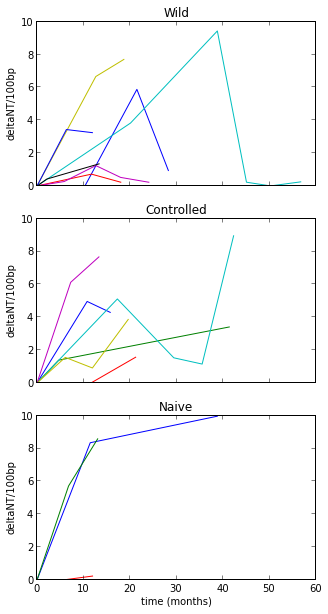
\includegraphics[width=0.7\textwidth]{VariationPlots_files/VariationPlots_fig_00.png}
\par
\end{center}
\end{codeoutput}
\end{codecell}
In the above figure I determined the number of mutations between
consecutive visits in both well controlled (left), uncontrolled patients
(middle) and naive patients (left). Each line represents a single
patient.

From these figures it looks like there is a roughly equal amount of
variation when you look at well controlled and uncontrolled patients. We
can also guess that in general there are bursts of genetic variation
which wanes over time. In the Controlled patient figure it looks like
all patients eventually return to a no-variation state but it takes 2-4
years of well controlled viral parameters for this to occur. To examine
this I'm going to look at consecutive pairs of visits (instead of
requiring 3+ visits) and then compare the results of consecutive
well-controlled visits to consecutive un-controlled visits.

\subsection{Data Extraction}
\begin{codecell}
\begin{codeinput}
\begin{lstlisting}
def pick_consecutive_visits(df):
    
    ndf = df.copy()
    ndf['ConsecutiveID'] = np.nan
    ndf['ConsecutiveType'] = ''
    
    idx = list(ndf.index)
    
    wc = list(ndf['VisitType'])
    
    gp_ind = 0
    tmp = []
    for (k_a, k_b), (wc_a, wc_b) in zip(zip(idx, idx[1:]), zip(wc, wc[1:])):
        if wc_a == wc_b:
            ndf['ConsecutiveID'].ix[[k_a, k_b]] = gp_ind
            ndf['ConsecutiveType'].ix[[k_a, k_b]] = wc_a
            tmp.append(ndf.ix[[k_a, k_b]].copy())
            gp_ind += 1
    
    if tmp:
        return concat(tmp, axis = 0, ignore_index = True)
    else:
        return None

odata = data.groupby('Patient ID', as_index=False).apply(align_pat_seq)
odata['MutPer100bp'] = 100*(odata['NumMut']/odata['NumCompare'])
cdata = odata.groupby('Patient ID', as_index=False)\
        .apply(pick_consecutive_visits)\
        .reset_index(drop = True).dropna()
print cdata
\end{lstlisting}
\end{codeinput}
\begin{codeoutput}
\begin{verbatim}
<class 'pandas.core.frame.DataFrame'>
Int64Index: 750 entries, 0 to 753
Data columns:
Patient ID         750  non-null values
VisitNum           750  non-null values
Date               750  non-null values
CD4                750  non-null values
VL                 750  non-null values
ART                750  non-null values
LTR                750  non-null values
VisitType          750  non-null values
NumCompare         750  non-null values
NumMut             750  non-null values
MutLoc             750  non-null values
Coverage           750  non-null values
MutPer100bp        750  non-null values
ConsecutiveID      750  non-null values
ConsecutiveType    750  non-null values
dtypes: float64(4), int64(2), object(9)
\end{verbatim}
\end{codeoutput}
\end{codecell}
\begin{codecell}
\begin{codeinput}
\begin{lstlisting}
def get_mut_rates(df):
    months = (df['Date'].max() - df['Date'].min()).days/30
    raw_mut = df['MutPer100bp'].ix[df.index[-1]]
    tser = Series([raw_mut, raw_mut/months], 
                    index = ['MutPer100bp', 'MutPer100bpPerMonth'])
    return tser

tmp = cdata.groupby(['Patient ID', 'ConsecutiveType', 'ConsecutiveID'])\
            .apply(get_mut_rates)

ntmp = tmp.groupby(level = ['ConsecutiveType', 'Patient ID'])\
            .apply(np.mean, axis = 0).dropna()
print ntmp.head()
\end{lstlisting}
\end{codeinput}
\begin{codeoutput}
\begin{verbatim}
MutPer100bp  MutPer100bpPerMonth
ConsecutiveType Patient ID                                  
controlled      A0001          3.063457             0.112352
                A0002          3.468934             0.353577
                A0004          0.829272             0.143554
                A0005          0.274725             0.013061
                A0008          3.224694             0.558259
\end{verbatim}
\end{codeoutput}
\end{codecell}
\subsection{Figures}
\subsubsection{Consecutive Variation Histogram}
\begin{codecell}
\begin{codeinput}
\begin{lstlisting}
fig, axes = plt.subplots(3,1, sharey = True, sharex = True, figsize = (5,10))
checks = ['wild', 'controlled', 'naive']

for ax, check in zip(axes.flatten(), checks):
    plt.sca(ax)
    hist_data = ntmp['MutPer100bp'].ix[check]
    plt.hist(hist_data.values, bins = 50, normed=True)
    plt.title(check)
    plt.ylabel('Frequency')

plt.xlabel('deltaNT/100bp')
plt.savefig('variation_hist.png')
\end{lstlisting}
\end{codeinput}
\begin{codeoutput}
\begin{center}
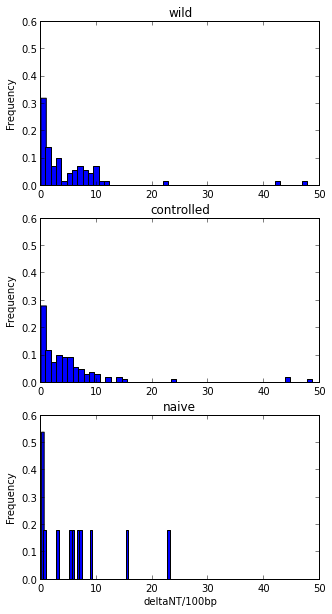
\includegraphics[width=0.7\textwidth]{VariationPlots_files/VariationPlots_fig_01.png}
\par
\end{center}
\end{codeoutput}
\end{codecell}
Again, even looking at the variation from consecutive visits I don't see
any difference between controlled visits, wild visits and naive visits.

\subsubsection{Paired Visits Table}
\begin{codecell}
\begin{codeinput}
\begin{lstlisting}
from scipy.stats import ttest_rel
paired_data = merge(ntmp.ix['wild'], ntmp.ix['controlled'], 
                    left_index = True, right_index = True,
                    suffixes = ('_Wild', '_Controled'))
print paired_data[['MutPer100bp_Wild', 'MutPer100bp_Controled']]
print paired_data[['MutPer100bp_Wild', 'MutPer100bp_Controled']].describe()

_, pval = ttest_rel(paired_data['MutPer100bp_Wild'], 
                    paired_data['MutPer100bp_Controled'])
print 'p-value:', pval
\end{lstlisting}
\end{codeinput}
\begin{codeoutput}
\begin{verbatim}
MutPer100bp_Wild  MutPer100bp_Controled
Patient ID                                         
A0004               2.273480               0.829272
A0015               0.000000               5.497522
A0019               9.621993               0.647948
A0037               0.201207               1.617251
A0044               5.973451               0.281599
A0062               5.894380               0.938086
A0067               0.000000               0.749064
A0096               9.042553               0.236407
A0113               0.000000               0.815217
A0145               0.562224               0.419287
A0162               0.775194               0.131579
A0284               3.339890               0.613276
       MutPer100bp_Wild  MutPer100bp_Controled
count         12.000000              12.000000
mean           3.140364               1.064709
std            3.614551               1.450787
min            0.000000               0.131579
25%            0.150905               0.384865
50%            1.524337               0.698506
75%            5.914148               0.856476
max            9.621993               5.497522
p-value: 0.125427074041
\end{verbatim}
\end{codeoutput}
\end{codecell}
In this paired data table I looked for patients which have both a Wild
and Controlled consecutive pair of visits. This limits our data but
takes into account a lot of the patient variablility issues. From the
data I don't see any drastic difference between the two populations.
While the p=0.125 does not mean that they are the same, it at least
means that they aren't likely to be different.

\subsubsection{Variation Boxplot}
\begin{codecell}
\begin{codeinput}
\begin{lstlisting}
fig, axes = plt.subplots(2,1, figsize = (7,7), sharex = True)

checks = ['wild', 'controlled', 'naive']
fields = [('MutPer100bp', 'deltaNT/100bp'),
          ('MutPer100bpPerMonth', 'deltaNT/100bp/month')]

for ax, (field, label) in zip(axes.flatten(), fields):
    plt.sca(ax)
    box_data = [ntmp[field].ix[c] for c in checks]
    plt.boxplot(box_data, sym = '', bootstrap = 1000);
    plt.xticks([1,2, 3], checks);
    plt.ylabel(label);

plt.savefig('variation_boxplot.png')
\end{lstlisting}
\end{codeinput}
\begin{codeoutput}
\begin{center}
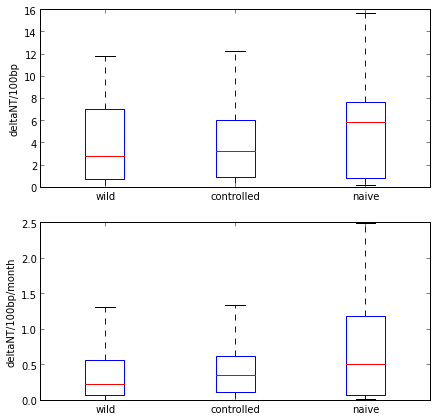
\includegraphics[width=0.7\textwidth]{VariationPlots_files/VariationPlots_fig_02.png}
\par
\end{center}
\end{codeoutput}
\end{codecell}
In order to examine whether the consecutive visits have a different
number of mutations per 100bp I made the above boxplots. There are 76
`wild' patients, 114 controlled and 12 naive patients. There clearly no
differences in the number of mututations on different therapy regmines.
The bottom plot normalizes the changes by the sampling time, just in
case there was an issue with one group going longer between visits.
Clearly not an issue.

\begin{codecell}
\begin{codeinput}
\begin{lstlisting}
cdict = {True:'b', False:'g'}
odata['MutPer100'] = 100*(odata['NumMut']/odata['NumCompare'])
plt.figure(figsize = (10,10))
types = [('naive', 'r'), 
         ('controlled', 'b'),
         ('wild', 'g')]
plt.hold(True)
for t, c in types:
    mask = odata['VisitType'] == t
    plt.scatter(odata['CD4'].ix[mask].values, 
                odata['MutPer100bp'].ix[mask].values, 
                alpha = 0.5, s = 20, color = c)

plt.xlim([0,2000]);
plt.ylim([0,50]);

plt.legend([t for t, _ in types]);
plt.xlabel('CD4 Count');
plt.ylabel('deltaNT/100bp');
\end{lstlisting}
\end{codeinput}
\begin{codeoutput}
\begin{center}
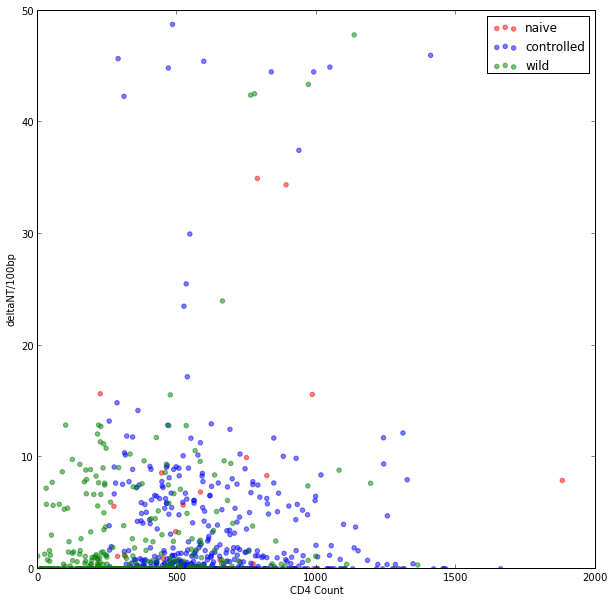
\includegraphics[width=0.7\textwidth]{VariationPlots_files/VariationPlots_fig_03.png}
\par
\end{center}
\end{codeoutput}
\end{codecell}
Looking at the correlation between CD4 and number of mutations. I do not
really see any relationship between CD4 count and number of mutations.
The outliers up there worry me a little, but there are roughly equal
numbers of each type.

\subsubsection{Coverage Map}
\begin{codecell}
\begin{codeinput}
\begin{lstlisting}
from collections import Counter
from itertools import chain

checks = ['wild', 'controlled', 'naive']
mask = cdata['Coverage'].map(len) == 634
fig, axes = plt.subplots(3,1, figsize = (10,10), sharex = True)

for typ, ax in zip(checks, axes.flatten()):
    
    plt.sca(ax)
    df = cdata[mask & (cdata['ConsecutiveType'] == typ)]
    covers = np.array([v for v in df['Coverage'].values])
    cover_map = np.sum(covers, axis = 0)/2
    #print cover_map
    plt.stackplot(range(634), cover_map, colors = 'k', alpha = 0.1)
    
    mut_counts = Counter(chain.from_iterable(df['MutLoc'].values))
    plt.bar(range(634), [mut_counts[m] for m in range(634)])
    plt.title(typ)
    
    plt.ylabel('Frequency')
plt.xlim([0, 634])
    
plt.xlabel('LTR position')    
plt.savefig('coverage_plots.png')
    
\end{lstlisting}
\end{codeinput}
\begin{codeoutput}
\begin{center}
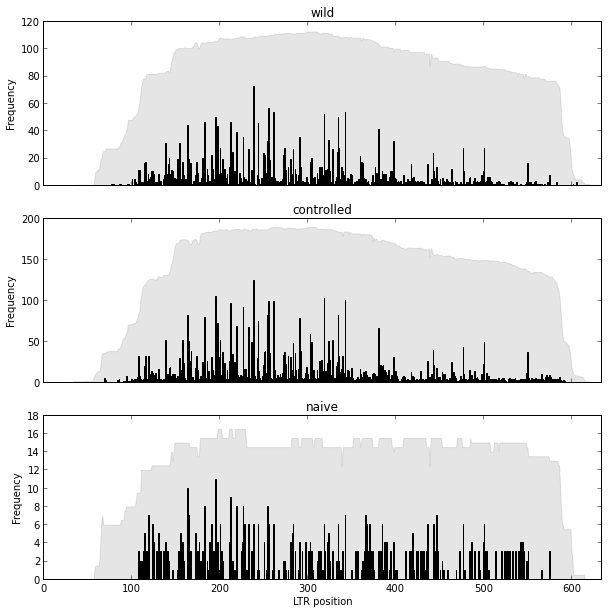
\includegraphics[width=0.7\textwidth]{VariationPlots_files/VariationPlots_fig_04.png}
\par
\end{center}
\end{codeoutput}
\end{codecell}
This is a set of coverage plots for the different populations. The grey
background represents the number of sequences at a particular LTR
position. The black bars represent the number of mutations found at each
position. You can see that we get the `normal' coverage for our
sequecing (we miss the beginnings and ends of the LTR). The mutations
are randomly distributed as far as I can tell.


\end{document}
